%input macros (i.e. write your own macros file called MacroFile1.tex)
%\include{Macros/MacroFile1}
\documentclass[oneside,12pt]{IIScthesisPSnPDF}
% \pagestyle{bfheadings}
%\usepackage{psfig}
% \usepackage{graphicx}
\usepackage{amssymb}
\usepackage{amsmath}
\usepackage{latexsym}
\usepackage{multicol}
\usepackage{booktabs}
\usepackage{multirow}
\usepackage{fancyhdr}
\usepackage[numbers]{natbib}
\usepackage{cleveref}
\usepackage{wrapfig}
\usepackage{algorithm}
\usepackage{algorithmic}
\usepackage{enumerate}
\usepackage{cancel}
\usepackage{mathrsfs}
% \usepackage{sfgame}
\usepackage{color}
\usepackage[compact]{titlesec}
\usepackage{mdwlist}
\usepackage{tikz}
\usepackage{varwidth}
\usepackage[vertfit]{breakurl}
\usepackage{datetime}
\usepackage{pdfpages}
% \usepackage{biblatex}
\usetikzlibrary{shapes,arrows, trees}
%This command reserves a whole page for a figure
%Its only argument is the caption
\newcommand{\fullpagefigspace}[2]{
\begin{figure}
\vspace{5.0in}
\caption{#1}
\label{#2}
\end{figure}
}
%            
%
\newcommand{\abs}[1]{$|{#1}|$}
\newcommand{\absq}[1]{$|{#1} |^{2}$}
\newcommand{\tabs}[1]{|{#1}|}
\newcommand{\tabsq}[1]{|{#1}|^2}
\newcommand{\half}{$\frac{1}{2}$}
\newcommand{\nth}{^{\mathrm{th}}}
\newcommand{\prob}[1]{\mathsf{Pr}\left(#1\right)}
\newcommand{\EXP}[1]{\mathsf{E}\!\left(#1\right)}
\newcommand{\D}{\displaystyle}
%%%%%%%%%%%%%%%%%%%%%%%%%%%%%%%%%%%%%%%%%%%%%%%%%%%%%%%%%%%%%%%%%%%%%%%%
%THE FOLLOWING IS FOR MAKING THE CAPTIONS IN SANS SERIF AND PUT A FIGRULE
%%%%%%%%%%%%%%%%%%%%%%%%%%%%%%%%%%%%%%%%%%%%%%%%%%%%%%%%%%%%%%%%%%%%%%%%
%\newcommand{\captionfonts}{\sf}

%\makeatletter  % Allow the use of @ in command names
%\long\def\@makecaption#1#2{%
%  \vskip\abovecaptionskip
%  \sbox\@tempboxa{{\captionfonts #1: #2}}%
%  \ifdim \wd\@tempboxa >\hsize
%    {\captionfonts #1: #2\par}
%  \else
%    \hbox to\hsize{\hfil\box\@tempboxa\hfil}%
%  \fi
%  \vskip\belowcaptionskip 
%  %\figrule{138mm}
%  }
%\makeatother   % Cancel the effect of \makeatletter
%%%%%%%%%%%%%%%%%%%%%%%%%%%%%%%%%%%%%%%%%%%%%%%%%%%%%%%%%%%%%%%%%%%%%%%%
%END OF MAKING THE CAPTIONS SANS SERIF
%%%%%%%%%%%%%%%%%%%%%%%%%%%%%%%%%%%%%%%%%%%%%%%%%%%%%%%%%%%%%%%%%%%%%%%%



\newcommand{\erf}[1]{
{\mbox{\mathsf{erf}}}\left( {#1} \right)
}

\newcommand{\erfc}[1]{
{\mbox{\mathsf{erfc}}}\left( {#1} \right)
}

\newcommand{\binomial}[2]{
\left(\! {{#1}\atop{#2}}\!\right)}

%Numbered environments
\newtheorem{remarks}{Remarks}[chapter] %\label{rmk:}
\newtheorem{example}{Example}[chapter] %\label{exp:}
\newtheorem{theorem}{Theorem}[chapter]
\newtheorem{lemma}{Lemma}[chapter]
\newtheorem{corollary}{Corollary}[chapter]
\newtheorem{discussion}{Discussion}[chapter] %\label{dis:}
\newtheorem{definition}{Definition}[chapter]
\newtheorem{proposition}{Proposition}[chapter]
\newtheorem{mechanism}{Mechanism}[chapter]
\newtheorem{question}{Question}[chapter]
\newtheorem{observation}{Observation}[chapter]
\newtheorem{fact}{Fact}[chapter]
\newcommand{\remove}[1]{}

\DeclareMathOperator*{\argmin}{\arg\!\min}
\DeclareMathOperator*{\argmax}{\arg\!\max}

\newenvironment{proof}{\noindent{\bf Proof:} \hspace*{1mm}}{\hfill $\Box$ }
\newcommand{\notes}[1]{}
\newcommand{\argument}[1]{\noindent{\bf Argument: }#1 \hfill $\Box$}
\newcommand{\VAR}[1]{\mathsf{Var}\!\left(#1\right)} 
\newcommand{\bmath}[1]{\mbox{\boldmath$#1$}}
\newcommand{\first}[1]{$1^{\mathrm{st}}$}
\newcommand{\second}[1]{$2^{\mathrm{nd}}$}
\newcommand{\qed}{\hfill \rule{2.5mm}{2.5mm}}
\def\QED{\mbox{\rule[0pt]{1ex}{1ex}}}
\def\Q{\hspace*{\fill}~\QED\par\endtrivlist\unskip}
\newcommand{\mech}{{\sc VCPM}}
\newcommand{\mechA}{{\sc MATRIX}}
\newcommand{\squishlisttwo}{
\begin{list}{$\blacktriangleright$}
{ \setlength{\itemsep}{0.5pt}
\setlength{\parsep}{0pt}
\setlength{\topsep}{0pt}
\setlength{\partopsep}{0.5pt}
\setlength{\leftmargin}{1em}
\setlength{\labelwidth}{1em}
\setlength{\labelsep}{0.5em} } }

\newcommand{\squishend}{
\end{list} }
\allowdisplaybreaks[1]


% \newcommand{\nobibentry}[1]{{\let\nocite\ignore\bibentry{#1}}}
\newdateformat{monthyeardate}{ \monthname[\THEMONTH], \THEYEAR}
\newcommand{\sn}[1]  {\noindent \textcolor{blue}{{\bf SN: }{``{\em #1}''}}}
\newcommand{\blankpage}{
\newpage
\thispagestyle{empty}
\mbox{}
\newpage
}

\newcommand{\blankpagewithnumber}{
\newpage
% \thispagestyle{empty}
\mbox{}
\newpage
}

\crefname{observation}{observation}{observations}
\crefname{algorithm}{algorithm}{algorithms}
\crefname{align}{equation}{equations}
\crefname{eqnarray}{equation}{equations}

% turn of those nasty overfull and underfull hboxes
\hbadness=10000
\hfuzz=50pt

% Put all the style files you want in the directory StyleFiles and usepackage like this:
% \usepackage{StyleFiles/watermark}

% Comment out the next line to get single spacing
\onehalfspacing

\begin{document}

\title{Secure Deduplication Across Files} 

\submitdate{\monthyeardate\today} 
\me
%\phd
%\mscengg
%\degree{Master of Engineering} 
\dept{Computer Science and Automation}
\faculty{Faculty of Engineering}
\author{Nithin V Nath}

% Using the watermark package which is in StyleFiles/
% and to remove DRAFT COPY ONLY appearing on the top of all pages comment out below line
%\watermark{DRAFT COPY ONLY}


\maketitle


\begin{center}
\LARGE{\underline{\textbf{Declaration of Originality}}}
\end{center}
\noindent I, \textbf{Nithin V Nath}, with SR No. \textbf{04-04-00-10-41-14-1-11158} hereby declare that
the material presented in the thesis titled

\begin{center}
\textbf{Secure Deduplication Across Files}
\end{center}

\noindent represents original work carried out by me in the \textbf{Deparment
of Computer Science and Automation} at \textbf{Indian Institute of
Science} during the years \textbf{2014-2016}.

\noindent With my signature, I certify that:
\begin{itemize}
	\item I have not manipulated any of the data or results.
	\item I have not committed any plagiarism of intellectual
	property.
	I have clearly indicated and referenced the contributions of
	others.
	\item I have explicitly acknowledged all collaborative research
	and discusions.
	\item I have understood that any false claim will result in severe
	disciplinary action.
	\item I have understood that the work may be screened for any form
	of academic misconduct.
\end{itemize}

\vspace{20mm}

\noindent {\footnotesize{Date:	\hfill	Student Signature}} \qquad

\vspace{20mm}

\noindent In my capacity as supervisor of the above-mentioned work, I certify
that the above statements are true to the best of my knowledge, and 
I have carried out due diligence to ensure the originality of the
report.

\vspace{20mm}

\noindent  {\footnotesize{Advisor Name: \textbf{Dr. Bhavana Kanukurthi} \hfill Advisor Signature}} \qquad



\blankpage

\vspace*{\fill}
\begin{center}
\large\bf \textcopyright \ Nithin V Nath\\
\large\bf \monthyeardate\today\\
\large\bf All rights reserved
\end{center}
\vspace*{\fill}
\thispagestyle{empty}

\blankpage

\vspace*{\fill}
\begin{center}
DEDICATED TO \\[2em]
\Large\it The Student Community\\[2em]
%\Large\it who can use and reuse this template to glory
\end{center}
\vspace*{\fill}
\thispagestyle{empty}

%\blankpage
%\includepdf[pages={1}]{declaration.pdf}

%\vspace*{\fill}
%\begin{tabular}{p{0.4\columnwidth}p{0.5\columnwidth}}
% {\em Signature of the Author}: & \dotfill \\
% & Your Name \\
% & Dept.\ of Computer Science and Automation \\ 
% & Indian Institute of Science, Bangalore \vspace{1in}\\
% {\em Signature of the Thesis Supervisor}: & \dotfill \\
% & Your Advisor's Name \\
% & Professor \\
% & Dept.\ of Computer Science and Automation \\ 
% & Indian Institute of Science, Bangalore
%\end{tabular}
%\vspace*{\fill}
%\thispagestyle{empty}

%\blankpage

%set the number of sectioning levels that get number and appear in the contents
\setcounter{secnumdepth}{3}
\setcounter{tocdepth}{3}

\frontmatter % book mode only
\pagenumbering{roman}


% \include{Dedication/dedication}
\prefacesection{Acknowledgements}
Firstly, I would like to express my sincere gratitude to my advisor Dr. Bhavana Kanukurthi for the continuous support of my research, for her patience, motivation, and immense knowledge. Her guidance helped me in all the time of research and writing of this thesis.
\\ \\
I thank my fellow labmates in Cryptography, Security and Privacy Group for the stimulating discussions, for the sleepless nights we were working together before deadlines, and for all the fun we have had.
\\ \\
Last but not the least, I would like to thank my family: my parents and my sister for supporting me throughout writing this thesis and my life in general.

\prefacesection{Abstract}
With cloud computing advances, more and more data is being stored in cloud storage. Deduplication
allows space savings for the cloud provider by storing only a single copy of repeating data.
Achieving this in a secure, privacy preserving way opens up several challenges. Traditional file-level deduplication allows space savings only when the files are identical to each other. In many scenarios, users upload files that are close to each other.
We discuss the construction of a secure deduplication scheme that enables deduplication not only for the files that are identical, but also for files that are close to one another under certain conditions\footnote{We divide the entire message space into codewords. Messages that come under the same codeword can be deduplicated easily}. We put forward a construction and proves its correctness and security.

\prefacesection{Publications based on this Thesis}
% \input{publications}

\tableofcontents
%\blankpagewithnumber
\listoffigures
\listoftables
%\blankpagewithnumber
% \printnomenclature  %% Print the nomenclature
% \addcontentsline{toc}{chapter}{Nomenclature}

\mainmatter % book mode only
\setcounter{page}{1}
\chapter{Introduction}
\label{chap:introduction}

Rise of cheap cloud storage solutions has encouraged users as well as enterprises to
resort to commercial cloud storage services such as Google Drive \cite{googleDrive} and 
Dropbox \cite{dropbox}. This has in turn triggered a large influx of data to be stored
in remote servers. In order to keep the prices competitive, service providers require
space saving techniques that can be deployed on a large scale without sacrificing
response time and reliability. In this setting, deduplication plays an important role \cite{practicaldedup}.
Deduplication is a well known technique that enables storage providers to store a single
copy of the data regardless of how many clients has uploaded the same data.
\\ \\
To see how a typical deduplication scheme works, imagine Alice uploads a file
$M$ to the server. Bob then requests to upload his copy of the same file $M$. The server identifies
that $M$ is already stored and simply updates the metadata associated with $M$ to show
that the file is owned by both Alice and Bob.
\\ \\
Based on the granularity of deduplication, two different flavours exist:
\begin{enumerate}
	\item \textit{File-level deduplication}: In this level, deduplication is
	exploited on the file level. Entire files are compared for deduplication
	which means only a single copy of each file will be stored.
	
	\item \textit{Block-level deduplication}: The files are divided into blocks and
	each block is checked for redundancy. This is more fine-grained and has its own
	advantages and disadvantages.
\end{enumerate}

Based on the deduplication architecture, there are two different strategies:
\begin{enumerate}
	\item \textit{Server-side deduplication}: Here the clients are oblivious to any of the
	underlying deduplication techniques. The file is uploaded to the server which
	may perform deduplication techniques. As far as the client is concerned, the upload and download
	functionalities work the same. This technique is also referred to as 
	\textit{target-based deduplication}
	
	\item \textit{Client-side deduplication}: In this technique, the client sends a \textit{tag}
	to the server before uploading the file. The \textit{tag} serves as a unique identifier of
	the entire data (e.g., a hash value) and is much shorter than the file. The server checks for
	redundancy and if a match occurs, the file is not sent over the network. Client-side also called
	\textit{source-based deduplication}, has the added advantage of saving network bandwidth.
\end{enumerate}
Deduplication along with privacy is a conflicting idea. On one hand, users will want
their data to be encrypted for a variety of reasons including personal privacy, corporate policy or
even legal reasons. On the other hand, 
the cloud providers would like to save space by identifying the file uploaded by 
the user and storing a single copy of the file.
Secure deduplication aims to resolve this conflict.	

\section{Motivation}
File level deduplication achieves significant space savings - as much as 75\% to 87\% depending 
on the file type \cite{practicaldedup}. Using deduplication,
cloud storage providers can save storage and thereby money which can in turn be transferred to
users in the form of cheaper storage options. By making deduplication compatible with privacy,
this can be achieved without the users having to sacrifice privacy.
\\ \\
Most of the existing deduplication schemes enables deduplication when files are identical. There
are several use cases when the files uploaded will be very close to each other. For instance, 
when a user uploads several photos which are taken quickly one after the other, the files
will be very close to one another. In this
paper, we put forward a scheme that can achieve deduplication across files. In this case, if a user
uploads a file to the server and a file that is close to this already exists in the server,
then the server will not store the entire file but a small piece (a $\Delta$) 
using which the original can be recovered later.


\section{Our Work}
\label{sec:intro}
This paper puts forward a scheme called $\scheme$ (deduplication across files) which enables deduplication even for files that are close to
each other. The basic idea is to divide the message space into several balls of same radius $\tau$
each with a message $\psi$. We use the hamming distance metric to do this. To encrypt a 
message $m$, it first is mapped to the corresponding $\psi$ that it belongs to. This $\psi$ is then
encrypted ($C_\psi$) and then uploaded along with a $\Delta$. $\Delta$ combined with $\psi$ will give
back the original message $m$. As long as the distance $\tau$ is small and the original
message has high enough entrpy, the $\Delta$ leaked will not compromise the security of the
encryption.\\ \\
To see that this enables deduplication, consider Figure \ref{fig:example}. Suppose Alice has
message $w_1$ that needs to be saved in the server. This will be uploaded to the server 
as encryption of $\psi$ ($C_\psi$) and $\Delta_1$. Later, Bob wants to upload $w_2$ and this
will be uploaded as $C_\psi$ and $\Delta_2$. The server needs to store only $\Delta_2$. Of course,
if Bob were also to upload $w_1$, deduplication is still achieved.

\begin{figure}[H]
	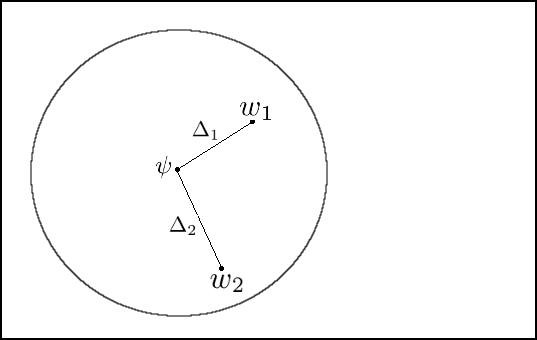
\includegraphics[scale=0.5]{example.png}
	\caption{Rectangle box represents the entire message space. Only one of many balls is shown}
	\label{fig:example}
\end{figure}



The rest of the paper is organised as follows: Section \ref{prelim} discusses the preliminaries needed 
and the ingredients that are used in this paper. Section \ref{sec:imle} explains Interactive MLE scheme
introduced in \cite{imle}, the adversarial model and the security game used. The construction of $\scheme$
is explained in section \ref{sec:constr} and its security is proved in section \ref{sec:res}.
% \chapter{Review}
\label{chap:review}

\begin{quote} \small
	We will briefly look at the related works in the Secure Deduplication field
\end{quote}

Douceur et al. \cite{convergentEnc} were the first to propose a novel deterministic cryptosystem
called \textit{convergent encryption} (CE) that enables deduplication to work with
encryption. The idea was to derive the encryption key from the message itself. This
will result in users possessing the same message to end up with the same ciphertext.
\\ \\
Halevi et al. \cite{proofOwner} identified several attacks that exploit client-side
deduplication and introduced the concept of proofs-of-ownership to mitigate these. This
work was extended to get a secure client-side deduplication by Xu et al. in \cite{weakLeakage}.
\\ \\
Bellare et al. in their 2013 paper \cite{mle} formalized the notions of security
in secure deduplication using a new cryptographic primitive called 
\textit{Message-Locked Encryption} (MLE) which subsumes CE. 
The paper was the first to formally argue
the security of secure deduplication and analysed the security of existing schemes as
well as put forward new practical security schemes.
\\ \\
In \cite{imle} Bellare et al. built upon MLE and put forward a new scheme they called
\textit{Interactive Message-Locked Encryption} (iMLE) in which upload and download are
protocols. They modelled privacy and security as games that enabled to argue for stronger notions
of security such as when an adversary controls multiple clients.
% \input{chap_skill_elicitation}
% \input{chap_resource_critical}
% \input{chap_team_formation}
% \input{chap_conclusions}

% \backmatter % book mode only
% \appendix
% \include{Appendix1/appendix1}
% \include{Appendix2/appendix2}

\bibliographystyle{plainnat}
%\bibliographystyle{Classes/CUEDbiblio}
%\bibliographystyle{Classes/jmb}
%\bibliographystyle{Classes/jmb} % bibliography style
% \renewcommand{\bibname}{References} % changes default name Bibliography to References
% \bibliography{References/references} % References file
\bibliography{references}
\end{document}
